\documentclass[answers]{exam}
\usepackage{../../template}
\author{niceguy}
\title{Problem Set 1}
\begin{document}
\maketitle
\begin{questions}

\question{Two small charged bodies are placed at two vertices of a square in free space (Figure \ref{1}). The electric force between the charges is stronger for}

\begin{figure}
	\centering
	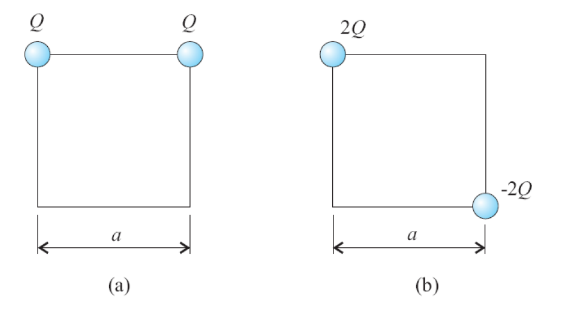
\includegraphics[width=0.7\textwidth]{1.png}
	\caption{Two small charged bodies}
	\label{1}
\end{figure}

\begin{solution}
	$$F = k\frac{Q_1Q_2}{r^2}$$
	Substituting, the forces are $k\frac{Q^2}{a^2}$ and $-k\frac{2Q^2}{a^2}$. The force is stronger in the second case.
\end{solution}

\question{Three point charges of unequal magnitudes and polarities are placed at vertices of an equilateral triangle (Figure \ref{2}). The electric force $\vec{F}_e$ on the lower right charge is}

\begin{figure}
	\centering
	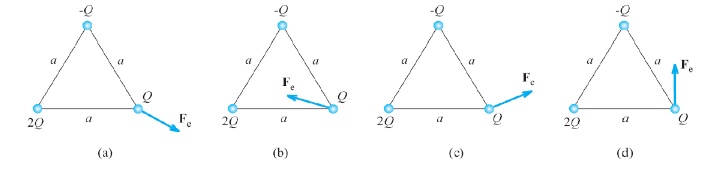
\includegraphics[width=0.7\textwidth]{2.png}
	\caption{Three point charges}
	\label{2}
\end{figure}

\begin{solution}
	Using vectors,
	\begin{align*}
		\vec{F}_e &= k\frac{2Q^2}{a^2}\hat{i} + k\frac{Q^2}{a^2}\left(-0.5\hat{i} + \frac{\sqrt{3}}{2}\hat{j}\right) \\
			  &= \frac{kQ^2}{a^2} \left(1.5\hat{i} + \frac{4+\sqrt{3}}{2}\hat{j}\right) \\
	\end{align*}
	Therefore, it is as in figure c.
\end{solution}

\question{Three point charges $Q = -1\unit{nC}$ are placed at three vertices $(a,0,0), (0,a,0)$ and $(0,0,a)$ of a cube with $a=1\unit{m}$. Find the electric field intensity vector at (a) the coordinate origin $(0,0,0)$ and (b) the point on the $z$-axis $(0,0,100\unit{m})$.}

\begin{solution}
	At the origin,
	$$\vec{E} = -k\frac{Q}{a^2}(\hat{i} + \hat{j} + \hat{k}) = 8.99\hat{i} + 8.99\hat{j} + 8.99\hat{k}$$
	On the $z$-axis,
	\begin{align*}
		\vec{E} &= -k\frac{Q}{10001}\left(\frac{1}{\sqrt{10001}}\hat{i} - \frac{100}{\sqrt{10001}}\hat{k} + \frac{1}{\sqrt{10001}}\hat{j} - \frac{100}{\sqrt{10001}}\hat{k}\right) + k\frac{Q}{9801}\hat{k} \\
			&= 8.99\times 10^{-6}\hat{i} + 8.99\times 10^{-6}\hat{j} - 2.71\times 10^{-3}\hat{k}
	\end{align*}
	This can also be done by approximating the point charges as 1 point charge $Q = -3\unit{nC}$ at $(0,0,0)$, which gives a similar result.
\end{solution}
\end{questions}
\end{document}
